\documentclass{beamer}
\usetheme{KUL}
\usepackage{multirow}
\usepackage{multicol}
\usepackage{tikz}
\usepackage{ulem}
\usepackage{siunitx}
\newcommand
\itemS{
\item[\textbf{\S}]}
\definecolor{darkgreen}{rgb}{0,0.598,0.199}
\usepackage{times} % set font on times new roman
\usepackage{eurosym} % package for Euro sign
\usepackage{lineno}   % package for line numbering
\usepackage{hyperref} % this is for url links
\usepackage{subcaption}  % this package enables one to put several
% figures next to each other
\usepackage{textcomp}
\usepackage{setspace}
\usepackage{gensymb}
\usepackage{url}
\usepackage[backend=biber,style=numeric-comp,sorting=none]{biblatex}
\addbibresource{bib.bib}

%----------------------------------
% Fill in the essential Information
%----------------------------------

\title[Candlestick Patterns]{Performance of candlestick patterns on
intraday market data}
\subtitle{Intermediate presentation}
\author[W.\ Notermans]{Wout Notermans} % between [] is short name,
% between {} is long name
\date{January 29, 2025} % Here you can also just type something, e.g.
% October 10, 2017
\institute[KU Leuven]{Faculty of Science\\ Department of
Mathematics\\ Section of Statistics and Data Science}

%----------------------------------
% ACTUAL PRESENTATION STARTS HERE
%----------------------------------

\begin{document}

% TITLE PAGE
{
  \setbeamertemplate{headline}{} %define local, empty header for title page
  \setbeamertemplate{footline}{} %define local, empty footer for title page
  \maketitle
}
\addtocounter{framenumber}{-1} % We don't count the title page

% \begin{kulblock}{Landslide}
%     A landslide is the downhill movement of soil mass
% \end{kulblock}

% ------------
% Introduction
% ------------

\section{Introduction}

\begin{frame}{Table of contents}
  \tableofcontents
\end{frame}

\begin{frame}[noframenumbering]{Table of contents}
  \tableofcontents[currentsection]
\end{frame}

\begin{frame}{Candlestick construction}
  \centering
  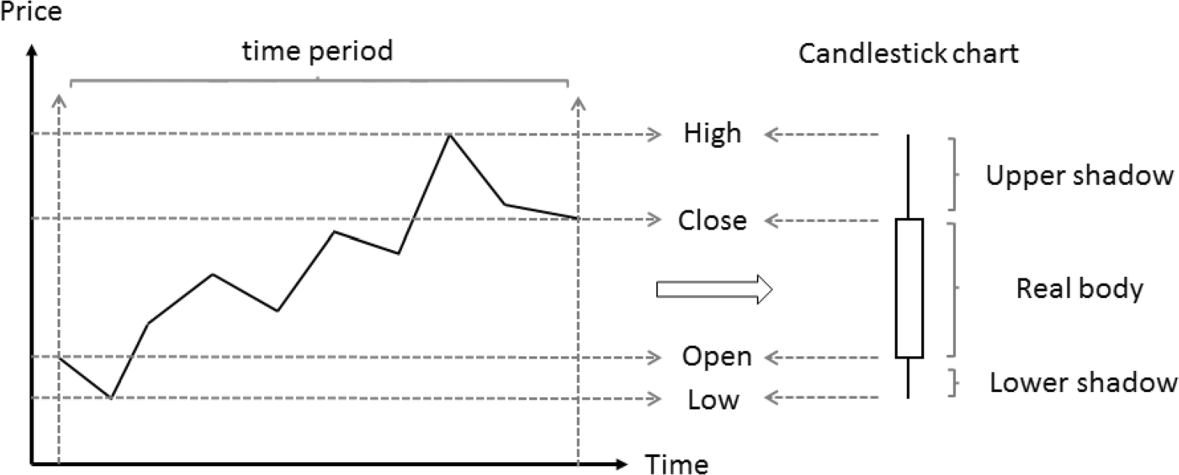
\includegraphics[width=\textwidth]{Images/candlestick_construction.png}
  Construction of a candlestick \cite{chen2020}.
\end{frame}

\begin{frame}{Candlestick pattern examples}
  \centering
  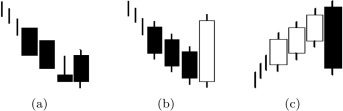
\includegraphics[width=\textwidth]{Images/pattern_example.jpg}
  (a) "Concealing Baby Swallow" (b) "Three-Line Strike, Bearish" (c) "Three-Line Strike, Bullish" \cite{hu2019}
\end{frame}

% -----------
% Methodology
% -----------

\section{Methodology}

\begin{frame}[noframenumbering]{Table of contents}
  \tableofcontents[currentsection]
\end{frame}

\begin{frame}{Data sets}
  \centering
  \begin{tabular}{|c|c|}
    \hline
    BND & Bonds \\ \hline
    GLD & Gold \\ \hline
    QQQ & Stocks \\ \hline
    SPY & Stocks \\
    \hline
  \end{tabular}\\[1em]
  Overview of the data sets.
\end{frame}

\begin{frame}{Data handling/preprocessing}
  \begin{itemize}
    \item Filtering pre/after-market
    \item Missing data $\rightarrow$ interpolation
    \item Aggregation
    \item Splitting of the data set
  \end{itemize}
\end{frame}

\begin{frame}{Calibration}
  \scalebox{0.8}{
    \begin{tabular}{cccccc}
      \hline
      & Doji & Short & Normal & Tall & Extremely tall \\
      Real body & $[0-10)$ & $[10-30)$ & $[30-70)$ & $[70-100]$ &  \\ \hline
      Shadow & $[0-10)$ & $[10-30)$ & $[30-70)$ & $[70-90)$ & $[90-100]$ \\ \hline
    \end{tabular}
  }
  \centering\\[1em]
  Percentiles of real bodies and shadows \cite{etschberger2006}.\\

  $$\text{Calculated as } |O-C|,\ H-\max\{O,C\},\ \min\{O,C\}-L.$$
\end{frame}

\begin{frame}{Calibration}
  \begin{itemize}
    \item Assumes length and color candle independent.
    \item Has to be checked $\rightarrow$ Kolmogorov-Smirnov test. \\ $$H_0: W = B \qquad H_1: W \neq B.$$ \\ Reject at 5\% significance.
  \end{itemize}
\end{frame}

\begin{frame}{Trend}
  \begin{itemize}
    \item Simple method to start: $\text{MA}(C_i,...,C_{i+5})$ monotonically increasing/decreasing 7 times.
  \end{itemize}
\end{frame}

\begin{frame}{Prediction}
  \begin{itemize}
    \item Typically classified as buy/sell signal.
    \item Evaluated according to prediction.
  \end{itemize}
\end{frame}

\begin{frame}{Evaluation}
  \begin{itemize}
    \item Buy/sell after pattern is detected.
    \item Make use of stop loss/take profit margins.
    \item Binomial test for winning rate. \\ $$H_0:\pi=0.5\qquad\qquad H_1:\pi>0.5$$
  \end{itemize}
\end{frame}

% -------
% Results
% -------

\section{Results}

\begin{frame}[noframenumbering]{Table of contents}
  \tableofcontents[currentsection]
\end{frame}

\begin{frame}{Detection results}
  \begin{itemize}
    \item Not many ``gapping" patterns.
    \item Some are rare due to stringent conditions.
    \item 103 $\rightarrow$ 63 patterns.
  \end{itemize}
  \centering
  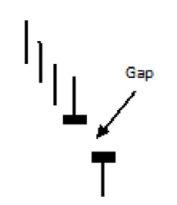
\includegraphics{Images/window_falling.png}
\end{frame}

\begin{frame}{BND results}
  \begin{itemize}
    \item No significant sell signals.
    \item Almost everything significant buy signal.
  \end{itemize}
\end{frame}

\begin{frame}{GLD results}
  \begin{itemize}
    \item Quite similar to BND.
    \item Some significant sell signals.
  \end{itemize}
\end{frame}

\begin{frame}{QQQ results}
  \begin{itemize}
    \item Again no significant sell signals.
    \item Level of significance lower than previous data sets.
    \item Some pattern behave the opposite now.
  \end{itemize}
\end{frame}

\begin{frame}{SPY results}
  \begin{itemize}
    \item Results similar to QQQ, indicates that results depend on asset type.
    \item Though not exactly the same, significance lost or gained.
  \end{itemize}
\end{frame}

\begin{frame}{Conclusion}
  \begin{itemize}
    \item Candlestick patterns appear to possess some significant predictive power.
    \item More buy than sell signals.
    \item Some patterns behave like the theory, some against it.
    \item Aggregation has little influence.
  \end{itemize}
\end{frame}

% -------------
% Looking ahead
% -------------

\section{Looking ahead}

\begin{frame}[noframenumbering]{Table of contents}
  \tableofcontents[currentsection]
\end{frame}

\begin{frame}{Looking ahead}
  \begin{itemize}
    \item Test different trend definitions, play with parameters.
    \item New methods of evaluation.
    \item Combinations with other aspects of technical analysis.
    \item Fuzzy approach.
    \item (Machine learning approach)
  \end{itemize}
\end{frame}

% ------------
% Bibliography
% ------------

\section*{Bibliography}

\begin{frame}[noframenumbering]
  \printbibliography
\end{frame}

\section*{}

\begin{frame}
  \begin{center}
    \color{cyan} \LARGE Questions?
  \end{center}
\end{frame}

\end{document}
